\chapter{Cellular Authentication}
Nelle reti cellulari passate\footnotemark(2G, 3G) gli aspetti di sicurezza vennero considerati in modo crescente ma non senza commettere errori e/o tralasciare aspetti fondamentali. Consideriamo qui aspetti e meccanismi di come un utente può autenticarsi in una rete cellulare e di come una stazione radio può confermare di essere valida. 
\footnotetext{Nella rete 1G la sicurezza non venne considerata affatto.}
\section{Rete 2G (GSM)}
In una rete GSM, le principali entità coinvolte in un processo di autenticazione sono le seguenti: 
\begin{itemize}
    \item \textbf{MS:} Mobile Sim (User). La sim contiene al suo interno una chiave segreta detta $K_i$\footnotemark, sconosciuta persino al dispositivo in cui la sim è inserita, così da poter non essere estratta.\footnotetext{Identity Key}
    \item \textbf{SN:} Serving Network (Visitor Location Register - VLR).
    \item \textbf{HN:} Home Network. E' l'unica a conoscere le chiavi $K_i$ degli utenti.
\end{itemize}
Quando un utente entra in rete, si avvia il seguente protocollo di autenticazione (\cref{fig:2gauth}): 
\begin{proposition}[2G Authentication]\label{prop:2gauth}
Assumiamo che l'utente abbia già notificato alla SN chi è e dove si trovi.
\begin{enumerate}
    \item La SN invia l'\textbf{IMSI}\footnotemark(identificatore dell'utente) e un \textbf{RAND} (sostanzialmente una challenge) alla \textbf{HN}.\footnotetext{\textsuperscript{\thefootnote}International Mobile Subscriber Identity}
    \item L'HN risponde con \textbf{SRES}\footnotemark(una response di tipo: H(RAND,$K_i$)) tramite un algoritmo $A3$ (una funzione hash) e un \textbf{encription key $K_C$} generata \textbf{dinamicamente} con l'algoritmo $A8$ a partire sempre da $K_i$ e \textbf{RAND}.\footnotetext{\textsuperscript{\thefootnote}Signed Result}
    \item La SN invia un'\textbf{authentication request} al MS inviando una nuova challenge \textbf{RAND} di 128bit.
    \item La MS crea una \textbf{authentication response} \textbf{SRES} da 32bit a partire dalla challenge di 128 e da $K_i$, tramite $A3$.
    \item La SN controlla se gli \textbf{SRES} corrispondono. In caso affermativo, consente l'accesso.
\end{enumerate}
\end{proposition}
Il punto di forza di questo protocollo di autenticazione è il concetto di \textit{\textbf{Key Derivation}}
\begin{definition}[Key Derivation]\label{def:keyderiv}
Concetto \textbf{fondamentale} con cui, a partire da una singola chiave che resta segreta per quasi\footnotemark ogni entità, è possibile generare delle nuove chiavi sempre diverse. 
\footnotetext{\textsuperscript{\thefootnote}Generalmente la chiave è codificata nell'hardware della scheda e salvata nel database dell'operatore.}
\end{definition}
\begin{figure}[ht]
    \centering
    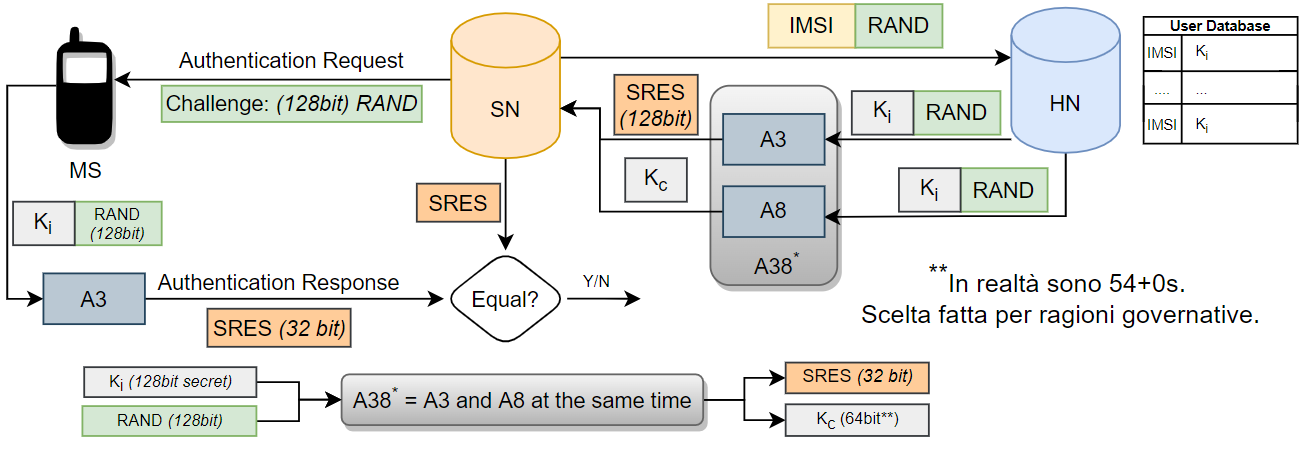
\includegraphics[width=\linewidth]{image/2gauth.png}
    \caption{2G Authentication Scheme}
    \label{fig:2gauth}
\end{figure}
\begin{corollary}[Authentication Vector]\label{cor:authvect}
Tripletta di valori generata dalla Home Network per consentire l'autenticazione di un utente nella rete.
\begin{equation*}
    \text{AuthVect}=\{\text{RAND}, \text{SRES}, K_c\}
\end{equation*}
\end{corollary}
Poiché in uno scenario reale un utente può autenticarsi molte volte in un lasso di tempo abbastanza breve, tipicamente il processo di auth viene ottimizzato \textbf{inviando alla SN una sequenza di authentication vector}. In questo modo, per $N$ richieste di auth la SN sarà da subito in grado di autenticare un utente, senza dover avviare lo scambio di messaggi con la HN.\\
Inoltre, viene ridotta anche la frequenza con cui una SN e la HN comunicano tra loro, riducendo l'impatto del processo sul traffico generale.
\subsection{Vulnerabilità delle reti GSM}
Nelle reti GSM la vulnerabilità principale è data dal fatto che il protocollo è \textbf{unilaterale} verso l'utente:
\begin{remark}
    \textbf{\textit{non abbiamo garanzie}}  sull'autenticità della service network/stazione radio base\footnotemark.
\end{remark}
\begin{proposition}[Rogue BTS Attack]
I sistemi GSM non supportano \textbf{mutua autenticazione}, rendendo possibile la creazione di una fake BTS con la quale generare dizionari di utenti che provano a connettersi e, volendo, autenticarsi al posto loro.
\end{proposition}
\footnotetext{In inglese BTS: base transceiver station}
Una possibile soluzione è quella di spostare la responsabilità di generare la challange alla home network, così che il fornitore stesso del servizio cellulare possa controllare l'autenticazione. In questo modo vengono inibiti attacchi basati sulla non affidabilità della SN e/o del canale tra SN e HN.\\
Una seconda vulnerabilità è dovuta al fatto che gli algoritmi di cifratura e derivazione (rispettivamente $A3$ e $A8$) erano algoritmi proprietari e, teoricamente, ogni operatore avrebbe dovuto implementare il proprio. Questo approccio è definito in gergo come:
\begin{definition}[Security by Obscurity]
\label{def:secbyobsc}
Filosofia di sicurezza per la quale un sistema è protetto semplicemente perché mantiene dei segreti sugli algoritmi che implementa.
\end{definition}
Ai tempi di GSM, gli operatori si misero d'accordo per implementare l'algoritmo \textit{COMP128}, considerato sicuro proprio perché non reso pubblico. Tuttavia, negli anni successivi l'algoritmo trapelò e violato in breve tempo.\\
\begin{remark}
Mai affidarsi per la sicurezza di algoritmo al fatto che questo possa essere privato perché prima o poi questo verrà bucato. E' fondamentale, invece, affidarsi agli esperti di crittografia e mai implementare soluzioni "fatte in casa".
\end{remark}
\begin{remark}
Riguardo alla dimensione effettiva del digest della chiave $K_c$, vennero standardizzati 64bit, suddivisi in 54 bit veramente sotto specifiche e una serie di zeri, in quanto a quei tempi nessuno era in grado di realizzare un attacco brute-force su una chiave di 54 bit (tantomeno su 64) se non i governi stessi, dotati di mezzi di calcolo più performanti.
\end{remark}
\section{Rete 3G (UMTS)}
Nella rete UMTS l'autenticazione è bilaterale \textit{(Mutual Auth \cref{chap:mutualauth})} e garantisce che i parametri usati nel processo siano sempre nuovi, evitando il riutilizzo di chiavi. Lo schema è il seguente:
\begin{proposition}[3G Authentication - AKA: Authentication and Key Agreement]\label{prop:3gauth}
Assumiamo che l'utente abbia già notificato alla SN chi è e dove si trovi.
\begin{enumerate}
    \item La SN invia l'IMSI del MS all'HN.
    \item\label{authvect5} L'HN invia $N$ authentication-vectors (\cref{cor:authvect}) fatti da quintuple, contententi:
    \[\{\text{RAND, XRES, CK, IK, AUTN}\}\]
    \begin{itemize}
        \item \textbf{RAND:} Authentication Challenge.
        \item $\textbf{XRES}=f_2(K,\text{RAND})$\textbf{:} Risultato atteso dalla CHAP-like authentication.
        \item $\textbf{CK}=f_3(K,\text{RAND})$\textbf{:} Cipher Key.
        \item $\textbf{IK}=f_4(K,\text{RAND})$\textbf{:} Integrity Key.
        \item $\textbf{AK}=f_5(K,\text{RAND})$\textbf{:} Authentication Key. Usato per mutual-authentication.
    \end{itemize}
    \item La SN inoltra a MS un \textbf{RAND} ed un \textbf{Autentication Number} definito come:
    \[\text{AUTN}=\{\text{SQN$\oplus$AK, AMF, MAC-A}\}\]
    \begin{itemize}
        \item \textbf{SQN:} Sequence Number (48bit).
        \item \textbf{AMF:} Auth\&Key Management Field (16bit). Specifica quale algoritmo o chiave da usare se ci sono scelte disponibili, finestra di sync e altri parametri. Utile per il cosiddetto \textbf{In-Band Signaling}.
        \item $\textbf{MAC-A}=f_1(K,\text{SQN, AMF, RAND})$\textbf{:} Message Auth Code permette all'MS di autenticare la rete (64bit).
    \end{itemize}
    \item Per autenticare la rete, MS esegue i seguenti passi:
    \begin{enumerate}
        \item genera la \underline{SUA} \textbf{AK} a partire dall'\textbf{AUTN} ricevuto.
        \item verifica la \textbf{"freschezza"} dell'informazione calcolando \textbf{SQN}$\oplus$\textbf{AK}$=$\textbf{SQN'} tale che:
        \[SQN'\in\text{\{SQN-MS+1, SQN-MS+\textbf{tollerance}\}}\]
        Dove \textbf{SQN-MS} è il contatore interno del MS mentre la tolleranza è utile a fini di resync in caso di messaggi persi.
        \item Se MS ha ricevuto un nonce valido, procede a rigenerare il \textbf{MAC-A}, verificando che sia uguale a quello ricevuto in \textbf{AUTN}. Se l'esito è positivo, invia la \textbf{RES} alla SN e aggiorna il valore del proprio sequence number come \textbf{SQN-MS $=$ SQN}.
    \end{enumerate}
    \item La SN confronta \textbf{RES} ed \textbf{XRES}, autenticando MS in caso affermativo.
\end{enumerate}
\end{proposition}
\begin{remark}
Gli algoritmi implementati all'interno della SIM sono $f_1,f_2,f_3,f_4.f_5$. Questi algoritmi sono \textbf{pubblici} e servono per derivare le chiavi necessarie all'autenticazione, tranne il primo che costituisce una funzione di criptaggio\footnotemark\, e il secondo che è sostanzialmente una funzione hash.
\footnotetext{$f_1$ è detta: \textbf{\textit{Actual Proof of Knowledge}} e certifica la conoscenza della chiave.}
\end{remark}
\begin{remark}
E' interessante osservare come il protocollo di \textbf{mutua autenticazione} usato \textbf{per validare la rete} è sostanzialmente basato su \textbf{un singolo messaggio}, quando ci aspetteremmo un protocollo di tipo \textit{3-way handshake} (3 messaggi). Analogamente, il meccanismo di \textbf{autenticazione del MS rispetto alla SN avviene come nella rete 2G} (\cref{prop:2gauth}).
\end{remark}
\begin{remark}
E' bene specificare che l'autenticazione della HN nei confronti della MS avviene tramite \textbf{sequence number (SQN)}, mantenuto in sincronizzazione tra le diverse parti della rete\footnotemark\, come \textbf{\textit{nonce implicita}}. Questo evita l'invio di un'ulteriore challenge da parte del MS alla HN.
\footnotetext{La Home Network mantiene il suo contatore nella variabile \textbf{SQN-HE}.}
\end{remark}
\begin{corollary}[Il ruolo dell'Anonymity Key]
L'AK viene utilizzata per \textbf{oscurare/mascherare}\footnotemark il sequence number in una fase in cui il \textbf{servizio di confidenzialità} non è ancora attivo. Ciò permette di risolvere il \textbf{Location Privacy Problem}, per il quale un attaccante può essere in grado di \textbf{determinare gli spostamenti di un utente tracciando incrementi del sequence number nella rete}.
\footnotetext{\textsuperscript{\thefootnote}Tramite $\oplus$.}
\end{corollary}
\subsection{(Pochi) Dettagli su IMSI-Catcher Attack}
Nel processo di auth (sia 3G che 2G) abbiamo supposto che l'utente si autentifichi una singola volta e, pertanto, che l'IMSI \textbf{venga inviato una sola volta nella rete}.
In condizioni normali è vero che viene inviato solo una volta l'IMSI dell'utente
Ma in generale, se ci dovessero essere errori di connessione o di autenticazione, la rete non può escludere l'utente e deve esserci un modo di recuperare la connessione. In quel caso, l'IMSI può essere inviato nuovamente, e potrebbe essere individuato.\\
Per evitare che l'IMSI venga catturato, forzandone un invio ripetuto magari tramite una rogue-BSS che disconnette l'MS, il protocollo impone che dopo la prima connessione venga usato sempre un IMSI \textit{temporaneo}: \textbf{TMSI}. Tale valore varia ogni volta, rendendo di fatto impossibile tracciare l'utente.

% inserire fig su 3g auth
% inserire fig sqn mask
% inserire fig su schema reti cellulari wireless dopo esonero
\subsection{(Pochi) Dettagli su Rete 4G/5G (LTE)}
La rete 4G (LTE) sfrutta lo stesso principio di autenticazione della rete 3G (UMTS), mentre la rete 5G sfrutta meccanismi molto più simili alle reti wi-fi, in quanto si pone l'obiettivo di fondere le tecnologie ed unificare le reti. 
\begin{remark}[Riguardo 5G]
Il meccanismo di \textbf{key-derivation} è migliorato. I moduli che dovrebbero garantire integrità in realtà non sono sempre implementati in quanto aggiungono molto carico di lavoro ed è stato fatto solo dal 4G in poi. Vi è inoltre una netta separazione per garantire protezione, detta \textbf{Security Edge Protecion} per separare la Serving Network dalla Home Network
\end{remark}
